\begin{figure}[t]
  \centering
  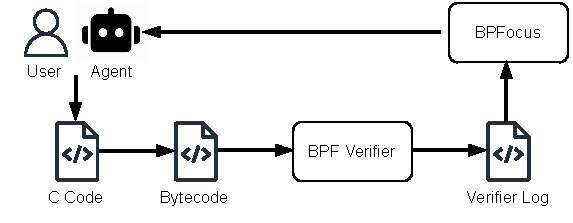
\includegraphics[width=0.96\columnwidth]{figures/sec-1-overview.pdf}
  \vspace{0.5pt}

  \noindent\textbf{\footnotesize (a) C Code}
  \begin{lstlisting}[style=bpfix,language=C,firstnumber=263]
if (ipv4_hdr)
    udph = (void *)ipv4_hdr + sizeof(*ipv4_hdr);
else
    udph = (void *)ipv6_hdr + sizeof(*ipv6_hdr);
if (udph + sizeof(struct udphdr) > data_end)  // bounds-checked
    return 1;

dst_port = __constant_ntohs(((struct udphdr *)udph)->dest); // rejected
  \end{lstlisting}

  \noindent\textbf{\footnotesize (b) Verifier Log}
  \begin{lstlisting}[style=bpflog]
from 31 to 34: ... R5_w=40 ...
; if (udph + sizeof(struct udphdr) > data_end) @ prog.c:267
35: (07) r3 += 8                      ; R3=48
36: (2d) if r3 > r2 goto pc+4         ; R2=pkt_end() R3=48
; dst_port = ...((struct udphdr *)udph)->dest; @ prog.c:270
37: (69) r2 = *(u16 *)(r5 +2)
R5 invalid mem access 'scalar'
  \end{lstlisting}

  \noindent\textbf{\footnotesize (c) \sys output}
  \begin{lstlisting}[style=bpfdiag]
error[BPFOCUS-E006]: verifier-visible compiler lowering hides the required proof
  = class: lowering_artifact
  = confidence: medium
  = next action: provenance
  --> prog.c:270
   |
263 | if (ipv4_hdr)
    | ------------- nearby source context for pointer provenance
267 | if (udph + sizeof(struct udphdr) > data_end)
    | -------------------------------------------- verifier state changes from pkt to scalar before the rejected access
270 | dst_port = __constant_ntohs(((struct udphdr *)udph)->dest);
    | ^^^^^^^^^^^^^^^^^^^^^^^^^^^^^^^^^^^^^^^^^^^^^^^^^^^^^^^^^^^ rejected here: verifier sees a scalar where a pointer is required
   |
   = verifier[229]: R5 invalid mem access 'scalar'
   = required proof: preserve a verifier-recognized pointer type at the operation that requires a pointer
help: Reacquire a verifier-tracked pointer before the rejected dereference.
help: Use the packet pointer that received the data_end proof, or rederive and recheck it before the load.
  \end{lstlisting}
  \caption{\sys on a real rejection (Stack Overflow 53136145). The verifier returns one register-level line; from the same log, \sys reconstructs the discarded proof and localizes the rejection to the point where the required proof was lost, mapping each span back to source.}
  \label{fig:overview}
\end{figure}